\documentclass[11pt]{article}

% Change "review" to "final" to generate the final (sometimes called camera-ready) version.
% Change to "preprint" to generate a non-anonymous version with page numbers.
\usepackage[preprint]{acl}
\usepackage{cuted}
% Standard package includes
\usepackage{times}
\usepackage{latexsym}
% Insert your packages here, for example:
\usepackage{booktabs}
% For proper rendering and hyphenation of words containing Latin characters (including in bib files)
\usepackage[T1]{fontenc}
% For Vietnamese characters
% \usepackage[T5]{fontenc}
% See https://www.latex-project.org/help/documentation/encguide.pdf for other character sets
\usepackage{makecell}
\renewcommand\theadfont{\bfseries}
\usepackage{tabularx}

% This assumes your files are encoded as UTF8
\usepackage[utf8]{inputenc}

% This is not strictly necessary, and may be commented out,
% but it will improve the layout of the manuscript,
% and will typically save some space.
\usepackage{microtype}

% This is also not strictly necessary, and may be commented out.
% However, it will improve the aesthetics of text in
% the typewriter font.
\usepackage{inconsolata}
\usepackage{cuted}
%Including images in your LaTeX document requires adding
%additional package(s)
\usepackage{graphicx}

\usepackage{amsmath}
\usepackage{amssymb}
\usepackage{array}
\usepackage{xcolor}      % For colored cells
\usepackage{colortbl}    % For table coloring
\usepackage{multirow}    % For merged cells
\usepackage{booktabs}
\usepackage{pifont}
\usepackage{cleveref}
\usepackage{tcolorbox}
\usepackage{makecell}
\usepackage{svg}
\usepackage{siunitx}
\usepackage{arydshln}
\usepackage{threeparttable}
\usepackage{wrapfig}
\usepackage[table]{xcolor}
\usepackage{hyperref}
\usepackage{url}
\usepackage{float}
\usepackage{placeins}
\usepackage{fontawesome5}
\usepackage{enumitem}
\usepackage[ruled,vlined,linesnumbered]{algorithm2e}
\usepackage{tikz}
\usepackage{stfloats}
\newcolumntype{L}[1]{>{\raggedright\arraybackslash}m{#1}}
\newcommand{\openailogo}{
\includegraphics[height=1.2em]{figure/openai.pdf}}
\newcommand{\qwenlogo}{
\includegraphics[height=1.2em]{figure/qwen_transparent_m.pdf}}
% If the title and author information does not fit in the area allocated, uncomment the following
%
%\setlength\titlebox{<dim>}
%
% and set <dim> to something 5cm or larger.
\newcommand{\memorybench}[1]{\textsc{MemoryBench}}
\newcommand{\longmemeval}[1]{\textsc{LongMemEval}}
\newcommand{\ours}[1]{TSM}

\definecolor{gptgray}{RGB}{245,246,248}
\definecolor{gptbar}{RGB}{230,232,236}
\definecolor{qwenlav}{RGB}{244,240,252}
\definecolor{qwenbar}{RGB}{228,220,246}
\newcommand{\gptgrayrow}[8]{%
  & \cellcolor{gptgray}#1
  & \cellcolor{gptgray}#2
  & \cellcolor{gptgray}#3
  & \cellcolor{gptgray}#4
  & \cellcolor{gptgray}#5
  & \cellcolor{gptgray}#6
  & \cellcolor{gptgray}#7
  & \cellcolor{gptgray}#8\\
}
\newcommand{\qwenlavrow}[8]{%
  & \cellcolor{qwenlav}#1
  & \cellcolor{qwenlav}#2
  & \cellcolor{qwenlav}#3
  & \cellcolor{qwenlav}#4
  & \cellcolor{qwenlav}#5
  & \cellcolor{qwenlav}#6
  & \cellcolor{qwenlav}#7
  & \cellcolor{qwenlav}#8\\
}


\title{Beyond Dialogue Time:\\ Temporal Semantic Memory for Personalized LLM Agents}

% Author information can be set in various styles:
% For several authors from the same institution:
% \author{Author 1 \and ... \and Author n \\
%         Address line \\ ... \\ Address line}
% if the names do not fit well on one line use
%         Author 1 \\ {\bf Author 2} \\ ... \\ {\bf Author n} \\
% For authors from different institutions:
% \author{Author 1 \\ Address line \\  ... \\ Address line
%         \And  ... \And
%         Author n \\ Address line \\ ... \\ Address line}
% To start a separate ``row'' of authors use \AND, as in
% \author{Author 1 \\ Address line \\  ... \\ Address line
%         \AND
%         Author 2 \\ Address line \\ ... \\ Address line \And
%         Author 3 \\ Address line \\ ... \\ Address line}

% \author{Miao Su \\
%   Affiliation / Address line 1 \\
%   Affiliation / Address line 2 \\
%   Affiliation / Address line 3 \\
%   \texttt{email@domain} \\\And
%   Second Author \\
%   Affiliation / Address line 1 \\
%   Affiliation / Address line 2 \\
%   Affiliation / Address line 3 \\
%   \texttt{email@domain} \\}

\author{
 \textbf{Miao Su\textsuperscript{1,2,3,4}},
 \textbf{Yucan Guo\textsuperscript{1,2,3}},
 \textbf{Zhongni Hou\textsuperscript{4}},
 \textbf{Long Bai\textsuperscript{1,2}},
\\
 \textbf{Zixuan Li\textsuperscript{1,2}},
 \textbf{Yufei Zhang\textsuperscript{4}},
 \textbf{Guojun Yin\textsuperscript{4}},
 \textbf{Wei Lin\textsuperscript{4}},
\\
 \textbf{Xiaolong Jin\textsuperscript{1,2,3}},
 \textbf{Jiafeng Guo\textsuperscript{1,2,3}},
 \textbf{Xueqi Cheng\textsuperscript{1,2,3}},
\\
 \textsuperscript{1}Institute of Computing Technology, Chinese Academy of Sciences\\
 \textsuperscript{2}State Key Laboratory of AI Safety\\
 \textsuperscript{3}School of Computer Science, University of Chinese Academy of Sciences\\
 \textsuperscript{4}Meituan
\\
 \small{
    \href{mailto:sumiao22z@ict.ac.cn}{sumiao22z@ict.ac.cn}
 }
}

\begin{document}
\maketitle
\begin{abstract}
Memory enables Large Language Model (LLM) agents to perceive, store, and use information from past dialogues, which is essential for personalization.
However, existing methods fail to properly model the temporal dimension of memory in two aspects: 1) Temporal inaccuracy: memories are organized by dialogue time rather than their actual occurrence time; 2) Temporal fragmentation: existing methods focus on point-wise memory, losing durative information that captures persistent states and evolving patterns. 
To address these limitations, we propose Temporal Semantic Memory (TSM), a memory framework that models semantic time for point-wise memory and supports the construction and utilization of durative memory.
During memory construction, it first builds a semantic timeline rather than a dialogue one. Then, it consolidates temporally continuous and semantically related information into a durative memory. During memory utilization, it incorporates the query’s temporal intent on the semantic timeline, enabling the retrieval of temporally appropriate durative memories and providing time-valid, duration-consistent context to support response generation.
Experiments on \textsc{LongMemEval} and \textsc{LoCoMo} show that \ours{} consistently outperforms existing methods and achieves up to 12.2\% absolute improvement in accuracy, demonstrating the effectiveness of the proposed method.

\end{abstract}

\section{Introduction}

\begin{figure}[t]
\centering
    % 上下结构放在第一页。。单栏。。。
    % 左：两条时间线，离散+duration；右，想做对问题，需要什么？ground truth+filter 跟motviation对应；具体做法忽略。。。

    % 举个例子：上现有方法；下认识；（根据intro的介绍顺序来）
    % 认识：两条时间线，离散+duration
    % 相关工作：时间怎么重要
    % 左右结构窄
    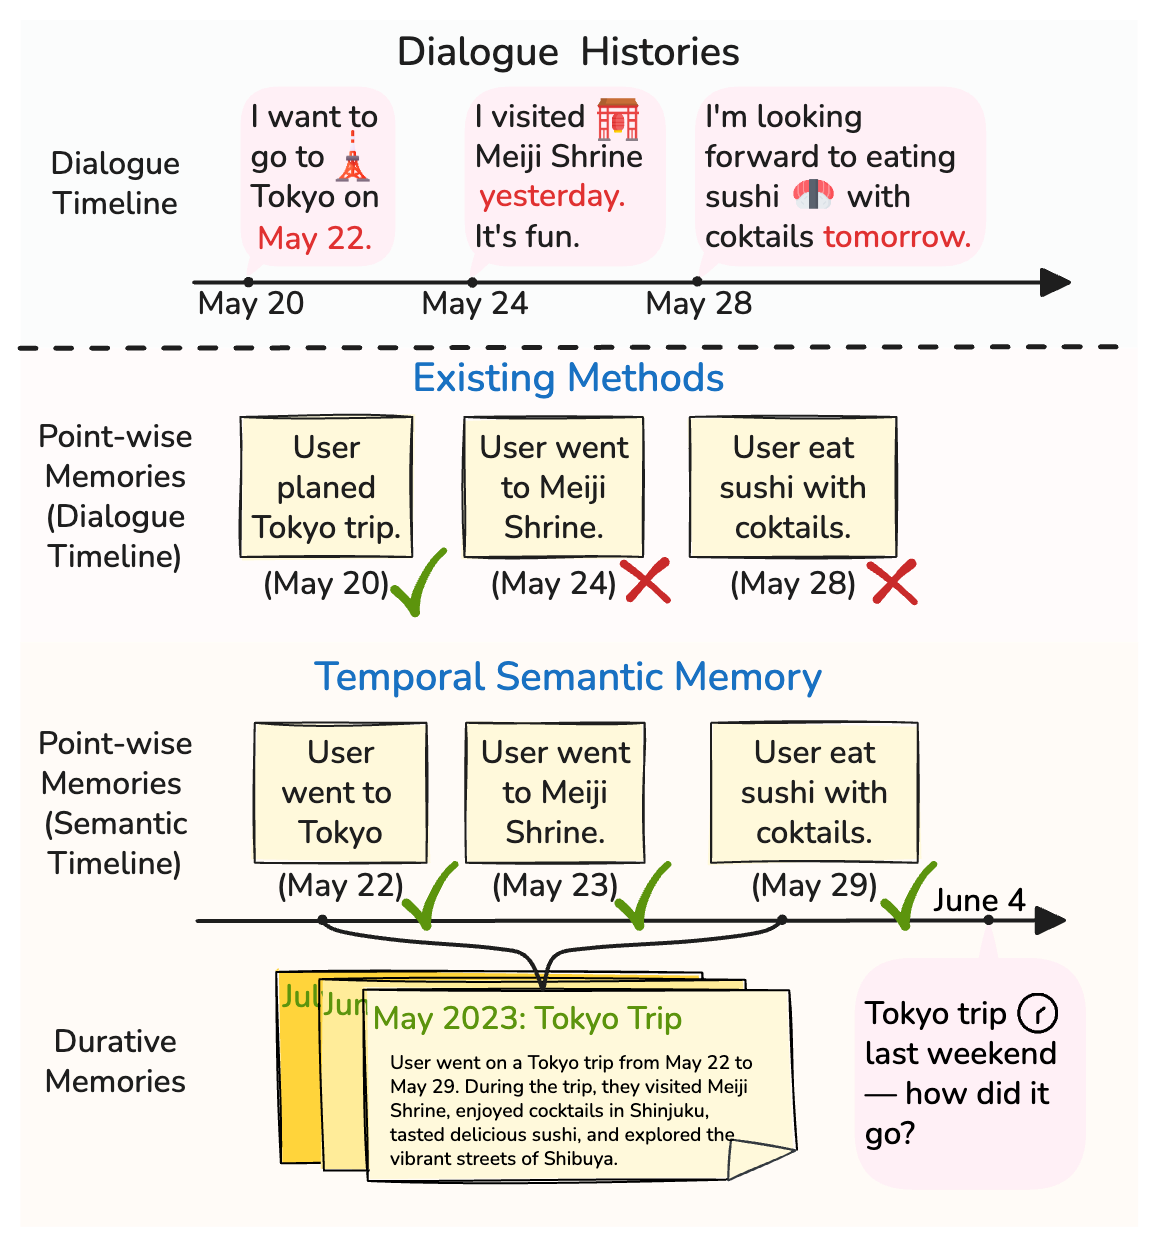
\includegraphics[width=\linewidth]{figure/intro.png}
    \caption{Comparison of existing methods vs. \ours{} with semantic timeline and durative memories.}
    \label{fig:motivation}
\end{figure}

Recent years have witnessed the rapid emergence of Large Language Model (LLM) agents, autonomous systems built upon LLMs with capabilities for reasoning, tool use, and long-term interaction~\cite{matarazzo_survey_2025,minaee_large_2025,luo_large_2025}. 
A key component of LLM agents is \textit{memory}. Instead of changing model parameters, memory provides an explicit store of interaction-derived information that agents can later reuse, enabling adaptation over extended interactions~\cite{sumers2023cognitive,wu_human_2025}. 
Personalized dialogue agents~\cite{chhikara2025mem0, li_hello_2025} exemplify this setting. Memory helps the agent maintain user-specific context, such as past plans, preferences, and evolving situations. 
It is typically implemented as a three-stage pipeline of construction, update, and utilization~\cite{hu_memory_2025}, so that responses remain coherent, grounded in prior interactions, and consistent over time.


Recent works construct memory by organizing dialogue histories into structured memory entries and retrieving them when needed~\cite{zhong_memorybank_2023, kim_pre-storage_2025, tan_prospect_2025, sun_hierarchical_2025}. 
However, as shown in~\Cref{fig:motivation}, existing methods suffer from two critical limitations in how they model temporal information.
(1) \textbf{Temporal inaccuracy.} Most systems treat the \emph{dialogue timeline} (when a chat turn is produced) as the primary temporal signal when assessing recency or relevance~\cite{rasmussen_zep_2025}. 
This is problematic because users often talk about events that occur at different times than the conversation itself, including future plans, past trips, and ongoing states. 
For example, when a user talks on May 28 about a trip happening on May 29, dialogue time and event time are misaligned; using the dialogue timeline alone can cause the system to store or retrieve memories under the wrong time context.
(2) \textbf{Temporal fragmentation.} Many methods store memories as isolated, point-wise entries~\cite{tan_prospect_2025, fang_lightmem_2025,chhikara_mem0_2025,rasmussen_zep_2025}. 
This representation breaks temporally continuous experiences into disconnected records, making it difficult to recover durations and long-term states.
For instance, the multiple entries within a week in~\Cref{fig:motivation} together describe a coherent Tokyo trip; treating them independently ignores their temporal continuity and semantic relatedness, which in turn hinders the formation of persistent states and evolving patterns.
Together, these issues prevent agents from retrieving complete and relevant memories, especially when the user query implicitly assumes a coherent real-world timeline.


In contrast, human memory relies on time as a scaffold for ordering and linking real-life experiences, supporting coherent recall across long-term memories~\cite{macdonald_hippocampal_2011,huet_episodic_2025}.
This highlights the importance of modeling time beyond a point-wise, dialogue-timeline view.
% Accordingly, we distinguish the \textbf{Dialogue timeline} (when chat turns occur) from the \textbf{Semantic timeline} (when described events happen and how long they last), exposing a fundamental mismatch between how memories are recorded and how user experiences are temporally structured.
% Moreover, explicitly modeling event \textbf{durations} enables temporally related mentions to be consolidated into higher-level, persistent representations (e.g., topics, preferences, and personas), rather than remaining as fragmented point-wise records.


To this end, we propose \textbf{Temporal Semantic Memory (TSM)}, a memory framework designed to support semantic-time grounded and duration-aware memory access.
In particular, \ours{} addresses the above challenges with two tightly coupled components:
(1) \textbf{Duration-aware memory construction.} TSM builds a \emph{semantic timeline} through a temporal knowledge graph, aligning memory with when events happen and how long they last.
Beyond recording point-wise facts, \ours{} links temporally continuous and semantically related mentions and consolidates them into \emph{durative summaries} that capture long-term states (i.e., topics and personas).
(2) \textbf{Semantic-time guided memory utilization.} During memory utilization, \ours{} incorporates the query's semantic temporal intent and retrieves memories at the appropriate temporal granularity, rather than relying on dialogue-time recency or semantics-only similarity that disregards timing.
This enables the system to return time-valid, duration-consistent context for response generation with correct temporal grounding.
In addition, \ours{} maintains memory with a lightweight hierarchical mechanism: it incrementally updates temporal facts online and periodically consolidates summaries to improve long-term consistency.

Extensive experiments on \textsc{LongMemEval}~\cite{wu_longmemeval_2025} and \textsc{LoCoMo}~\cite{maharana_evaluating_2024} demonstrate that \ours{} consistently outperforms strong memory baselines, with the largest gains on multi-session understanding and temporal reasoning tasks, validating the effectiveness of semantic-time grounding and duration-aware consolidation.

\section{Related Work} 

\subsection{Agent Memory}

LLM agents are increasingly equipped with long-term memory that grows and adapts over time, allowing them to accumulate knowledge, recall prior context, and adjust behavior based on experience~\citep{owl2025, openmanus2025, google2025deepresearch, bytedance2025deerflow}. There are several functions of agent memory: 
Factual memory stores persistent information such as user profiles, dialogue history, and world facts to support long-term consistency and personalization, as explored in memory-augmented dialogue agents and long-term user modeling systems~\citep{park_generative_2023, packer_memgpt_2024,nan_nemori_2025,kwon_embodied_2025};
experiential memory records past interaction trajectories and distilled strategies to enable continual self-improvement across tasks, exemplified by case-based, strategy-based, and skill-based learning in reflective and self-improving agents~\citep{shinn2023reflexion,yan_memory-r1_2025,zhou_mem1_2025,ouyang_reasoningbank_2025};
working Memory provides mechanisms for the active management of transient context~\cite{zhou_mem1_2025,zhang_memgen_2025}.

In this work, we focus on user-specific factual memory to support temporally grounded, personalized agent over long-term interactions.

\subsection{Graph-structured Memory }
In the context of agent memory, graph-structured memory arises naturally when agents accumulate relational insights over time. %Graph RAG systems structure the knowledge base as a graph and leverage graph traversal or graph-based ranking algorithms to retrieve context~\cite{peng_graph_2024}. 
Mem0$^{g}$ employs a scalable two-phase architecture (extraction and update) that dynamically stores and retrieves salient facts in a knowledge graph~\cite{chhikara2025mem0}.
A-MEM~\cite{xu2025mem} builds an interconnected memory network inspired by Zettelkasten~\cite{kadavy_digital_2021}, where each new memory is represented as a structured note with attributes (e.g., keywords/tags), and the system dynamically links related memories and updates existing notes as new information arrives, enabling an evolving memory graph.
Zep~\cite{rasmussen_zep_2025} proposes a temporal knowledge graph memory layer, emphasizing temporal reasoning over an evolving graph rather than static document retrieval. However, it ignores time during the memory retrieval stage. Other recent systems (e.g., G-memory~\cite{zhang_g-memory_2025}) similarly allow the internal graph to be constructed, extended, or reorganized throughout the agent's operation.

Many prior graph-based memory systems primarily treat the graph as a persistent store of extracted facts, but the \emph{evolution} of memory in a time period is not considered, yet the retrieval stage still underutilizes the \emph{semantic time} encoded in the graph, resulting in temporally misaligned recall.



\section{Methodology}

\begin{figure*}
    \centering
    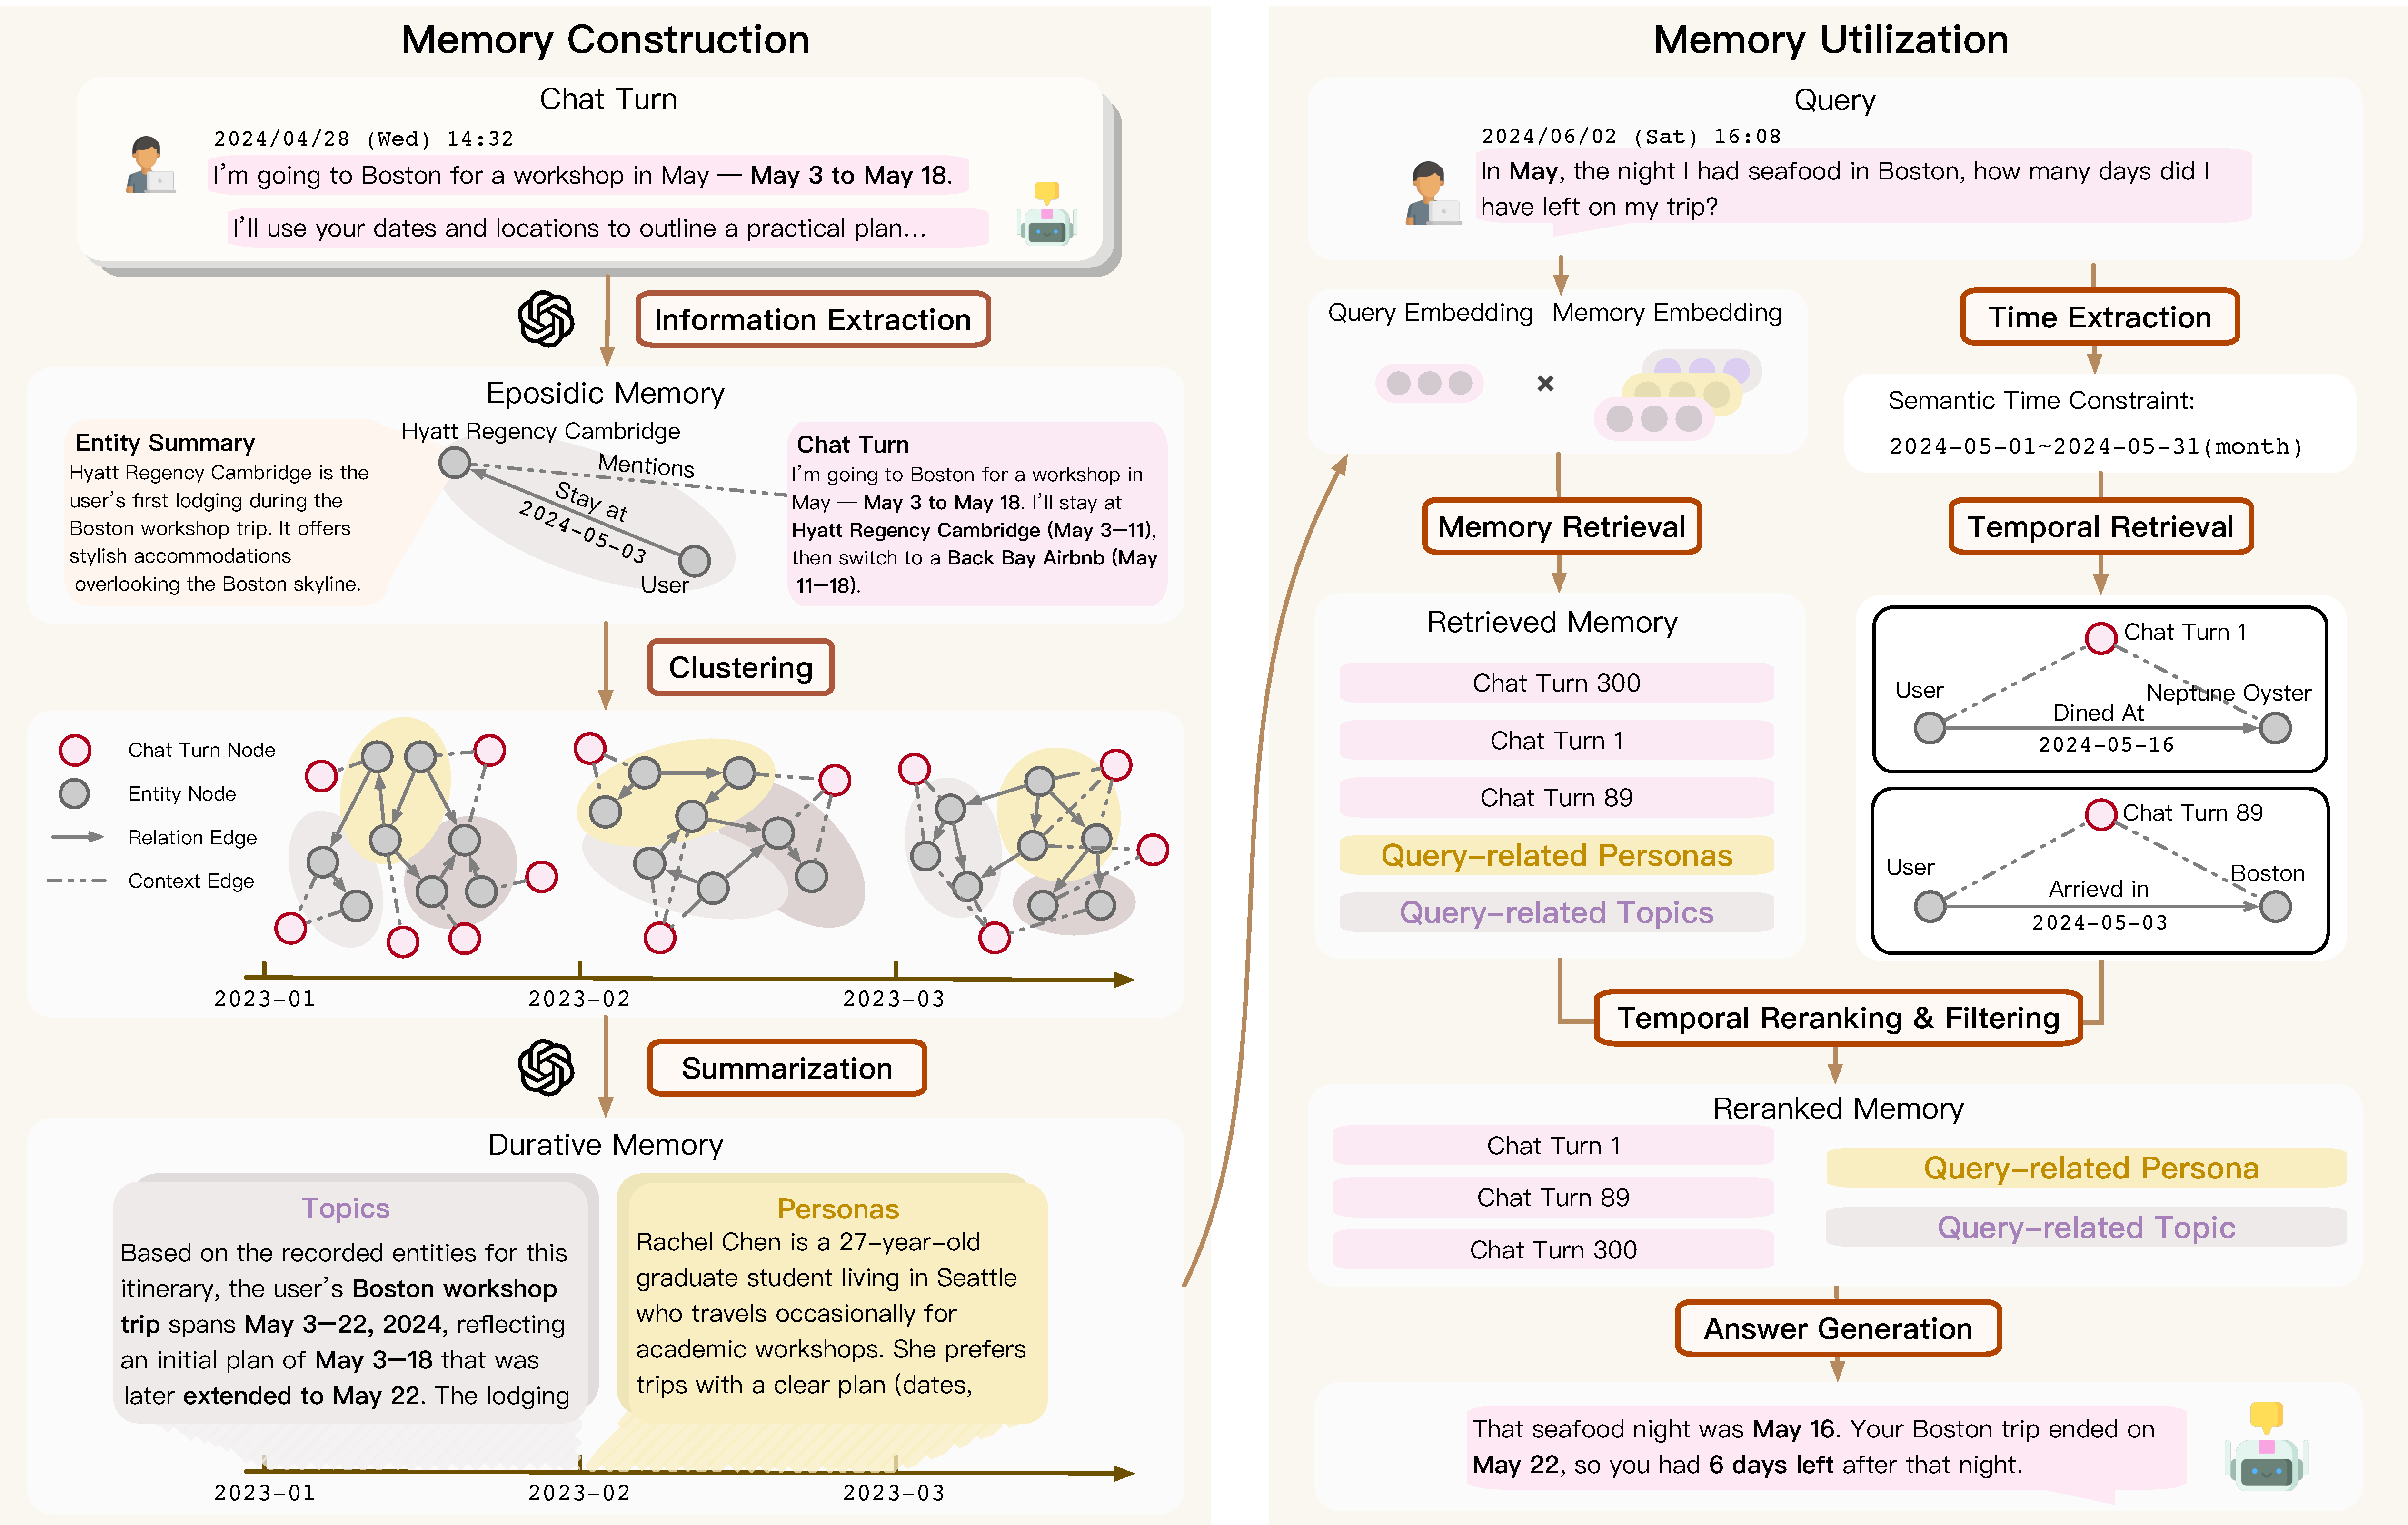
\includegraphics[width=\textwidth]{figure/Method.pdf} 
    \caption{The overall framework of \ours{}. Memory consolidation constructs a temporal knowledge graph from episodic memory and subsequently consolidates it into time-aware durative memory. Memory utilization retrieves accurate memories by applying semantic-temporal constraints.} 
    \label{fig:framework}
    
\end{figure*}

\subsection{Preliminary}
We consider the task of building a personalized dialogue agent in a \textbf{multi-session} conversational setting.
A \textit{session} represents a distinct interaction period, often delimited by user inactivity, explicit user confirmation of conversation completion, or the initiation of a new dialogue thread.
Within each session, the conversation unfolds as a sequence of chat turns, where a \textit{chat turn} consists of a user query and the agent's corresponding response.

% Formally, a standard agent memory system consists of two parts: a parametric memory $\theta$ (e.g., the backbone LLM) and a non-parametric memory $M$ (e.g., an external memory base).

Typically, a standard agent memory system implements three core functions: 

(1) Construction, which transforms raw chat history $D$ into structured memory $M$,
\[
M = f_{\text{construct}}(D)
\]

(2) Update, which refines the existing memory with new conversational data $D'$,

\[
M' = f_{\text{update}}(M,D')
\]


(3) Utilization (Retrieval), which generates an answer $A$ to a given query $Q$ based on the stored memory,
\[
A = f_{\text{retrieve}}(M,Q).
\]


\subsection{Overview}
% The concept of memory in intelligent systems has been extensively studied in the fields of both neural science, social science, and computer science. For example, previous studies have compared their components with neurobiological analogs for human memory (HippoRAG2). 
% Building on these insights, we draw inspiration from hippocampal and prefrontal cortical structures to design our system’s memory storage: a knowledge graph capturing contextual and associative information, analogous to the hippocampus, and a hierarchical tree consolidating and abstracting knowledge over time, analogous to the prefrontal cortex.

% In humans, the hippocampus and prefrontal cortex jointly support memory encoding and consolidation. 

As illustrated in Figure~\ref{fig:framework}, \ours{} consists of two stages: Memory Construction (\S\ref{sec:construction}) that builds a temporal knowledge graph as a episodic memory and organizes episodic interactions into durative memories; Memory Utilization (\S\ref{sec:retrieval}) that performs constraint-aware retrieval by integrating dense matching with temporal reranking and filtering for accurate memory access. Additionally, we build an Update Mechanism (\S\ref{sec:update}) that periodically refreshes both the episodic memory and the constructed durative memory to ensure long-term consistency.  


% The hippocampus rapidly binds contextual and relational information into episodic traces, while the prefrontal cortex gradually abstracts and stabilizes these traces into long-term semantic structures. [Baddeley’s Working Memory Model (1986)]

% Notably, recent research (Geva-Sagiv et al., 2023, Nature Neuroscience) shows that enhancing hippocampal–prefrontal synchrony during sleep strengthens declarative memory consolidation, highlighting their cooperative role in transforming transient experiences into long-term memory. % todo todo todo，这能和什么对应, retrieval?

% a figure here

\subsection{Duration-aware Memory Construction}
\label{sec:construction}
We construct two complementary memory types from dialogue streams through a hierarchical process:

\noindent\textbf{Episodic Memory} captures atomic facts with specific semantic timestamp (e.g., "visited Tokyo on May 23"), organized as a temporal knowledge graph with explicit temporal grounding.

\noindent\textbf{Durative Memory} maintains enduring patterns that persist across extended periods, derived from episodic memory through temporal segmentation and semantic abstraction. Unlike event-specific episodic memories, durative memories represent stable user characteristics (e.g., sustained interests, evolving preferences) extracted from accumulated experiences. This concept parallels semantic memory in cognitive science.

\subsubsection{Episodic Memory Construction}

We construct a Temporal Knowledge Graph (TKG) as a structured memory index that records episodic information mentioned in the dialogue history following Zep~\cite{rasmussen_zep_2025-1}. The TKG is not directly used as retrievable memory content; instead, it provides precise temporal localization and semantic time access for subsequent memory construction and retrieval.

Formally, the TKG is defined as a set of temporally grounded facts
\begin{equation}
\mathcal{G} = \{ (e_s, r, e_o, t) \mid t \in \mathbb{T} \}.
\end{equation}
where $e_s$ and $e_o$ denote the subject and object entities, $r$ denotes a semantic relation, and $t$ denotes the time point when the fact is valid.

In addition to temporal facts, each entity node maintains a compact entity summary extracted from its supporting dialogue contexts. We represent an entity as $e \triangleq (n_e, s_e),$ where $n_e$ is the canonical entity name and $s_e$ is an LLM-generated entity summary that consolidates salient attributes of $e$.

We extract entities and relations from each turn (with a context window of the preceding $n$ turns) and incrementally integrate them into the TKG via deduplication and temporal consistency checks (details in Section~\ref{sec:update}).

The resulting TKG serves as an episodic memory index that supports time-aware access, temporal filtering, and consistency checking, while deferring semantic abstraction to later stages.

\subsubsection{Durative Memory Construction}

Based on the episodic memory graph, we construct durative memory by aggregating episodic information into higher-level semantic representations. 

Given the temporal knowledge graph, we partition it into a sequence of temporal slices
\begin{equation}
\begin{aligned}
\mathcal{G} &= \bigcup_{k} \mathcal{G}^{(k)}, \\
\mathcal{G}^{(k)} &= \{ (e_s, r, e_o, t) \mid t \in [\tau_k, \tau_{k+1}) \},
\end{aligned}
\end{equation}
where $[\tau_k, \tau_{k+1})$ denotes a fixed temporal interval. In our implementation, the granularity is set to one month by default.

For each temporal slice $\mathcal{G}^{(k)}$, we collect the involved entity set
\begin{equation}
\mathcal{E}^{(k)} = \{ e \mid e \text{ appears in } \mathcal{G}^{(k)} \}.
\end{equation}


We apply a Gaussian Mixture Model (GMM)~\cite{huang_retrieval-augmented_2025} to cluster entities within the same temporal slice
\begin{equation}
p(z \mid e) = \mathrm{GMM}(\mathbf{h}^{\mathrm{name}}_e),
\end{equation}
where $z$ denotes a latent cluster capturing a coherent semantic theme. For each entity $e$, we assign it to the most likely cluster $a(e)=\arg\max_{z} p(z\mid e)$, and define
\begin{equation}
\mathcal{E}_z = \{ e \in \mathcal{E}^{(k)} \mid a(e)=z \}.
\end{equation}

For each cluster $z$ in the $k$-th temporal slice, let
\begin{equation}
\mathcal{X}_z = \{ (n_e, s_e) \mid e \in \mathcal{E}_z \}
\end{equation}
denote the entity-summaries in the cluster. We define a topic as
\begin{equation}
\begin{aligned}
\mathrm{Topic}_z &= \{ \tau_k, s_z, \mathbf{c}_z \}, \\
s_z &= \mathrm{LLM}_{\mathrm{sum}}(\mathcal{X}_z), \\
\mathbf{c}_z &= \mathrm{Embedding}(s_z),
\end{aligned}
\end{equation}
where $\tau_k$ denotes the corresponding time slice, $s_z$ is the textual topic summary, and $\mathbf{c}_z$ is its embedding used for downstream retrieval.

To capture user-level characteristics, we further aggregate the dialogue contexts associated with the entities in $\mathcal{E}_z$. Using a bidirectional index between entities and their originating chat turns, we collect the corresponding dialogue
\begin{equation}
\mathcal{D}_z = \{ d \mid d \text{ mentions } e,\; e \in \mathcal{E}_z \}.
\end{equation}

The persona representation is defined as
\begin{equation}
\begin{aligned}
\mathrm{Persona}_z &= \{ \tau_k, \mathbf{p}_z, \mathbf{u}_z \}, \\
\mathbf{p}_z &= \mathrm{LLM}_{\mathrm{sum}}(\mathcal{D}_z), \\
\mathbf{u}_z &= \mathrm{Embedding}(\mathbf{p}_z),
\end{aligned}
\end{equation}
where $\mathbf{p}_z$ captures stable user traits, preferences, and behavioral patterns expressed within the temporal slice, and $\mathbf{u}_z$ denotes its embedding.

Through temporal segmentation and semantic abstraction, the constructed topics and personas form hierarchical, temporally anchored durative memory. It captures durative user states beyond isolated point events, thereby supporting efficient long-term storage and subsequent constraint-aware retrieval.


\subsection{Semantic-time Guided Memory Utilization}
\label{sec:retrieval}
This stage retrieves memory that is both semantically relevant and temporally consistent with the user query. Given a query $q$, we (i) infer its semantic time constraint $T_q$, (ii) perform dense retrieval over topics, personas, and raw dialogue chunks, and (iii) enforce the temporal constraint by filtering time-anchored summaries and promoting candidates supported by temporally valid evidence from the TKG.

Given a user query $q$ issued at time $t_{\mathrm{now}}$, we first parse its semantic-time constraint $T_q$, i.e., the time range when the described event is intended to hold (rather than the dialogue time)
\begin{equation}
T_q = \mathrm{ParseTime}(q, t_{\mathrm{now}}),
\end{equation}
where $\mathrm{ParseTime}(\cdot)$ is implemented with spaCy~\cite{Honnibal2020spaCy} and resolves both explicit and relative time expressions.

Let the retrievable memory pool be
\begin{equation}
\mathcal{M} = \mathcal{M}_{\mathrm{topic}} \cup \mathcal{M}_{\mathrm{persona}} \cup \mathcal{M}_{\mathrm{raw}},
\end{equation}
where each topic/persona entry $m$ carries a slice timestamp $\tau(m)$ from construction, while each raw segment $m \in \mathcal{M}_{\mathrm{raw}}$ is a chat turn. We compute dense retrieval scores 
\begin{equation} s_{\mathrm{sem}}(m;q) = \mathrm{sim}\big(\mathrm{Enc}(q), \mathrm{Enc}(m)\big), \end{equation} 
and retrieve Top-$K$ candidates \begin{equation} \mathcal{D} = \mathrm{TopK}_{m \in \mathcal{M}} \; s_{\mathrm{sem}}(m;q). 
\end{equation}

To align retrieval with the temporal intent in $q$, we apply temporal filtering to the retrieved topics/personas (post-retrieval in our implementation):
\begin{equation}
\mathrm{Keep}(m,T_q)=
\begin{cases}
\mathbb{I}\!\big[\tau(m) \in T_q\big], &
\begin{aligned}[t]
m \in \mathcal{M}_{\mathrm{topic}}\\
\cup\ \mathcal{M}_{\mathrm{persona}},
\end{aligned}\\[4pt]
1, & m \in \mathcal{M}_{\mathrm{raw}}.
\end{cases}
\end{equation}

In parallel, we query the TKG for temporally valid facts and map them to their originating  chat turns via the bidirectional index:
\begin{equation}
\begin{aligned}
\mathcal{F}_T &= \{ (e_s,r,e_o,t)\in \mathcal{G} \mid t \in T_q \}, \\
\mathcal{S}_T &= \mathrm{Idx}(\mathcal{F}_T).
\end{aligned}
\end{equation}

where $\mathrm{Idx}(\cdot)$ returns the set of raw chat turns linked to the facts.

Finally, we rerank candidates through a composite scoring function that prioritizes semantic-time alignment before semantic similarity. To be specific, we use the indicator $\mathbb{I}[\tau(m)\in T_q]$ as the primary key and $s_{\mathrm{sem}}(m;q)$ as the secondary key:
\begin{equation}
\pi(m;q)=\Big(\mathbb{I}\big[\tau(m)\in T_q\big],\ s_{\mathrm{sem}}(m;q)\Big),
\end{equation}
and sort candidates in descending lexicographic order of $\pi(\cdot)$:
\begin{equation}
\mathcal{R}=\mathrm{Sort}_{m\in\mathcal{D}}\ \pi(m;q).
\end{equation}

This design enforces the query time constraint on compact summaries (topics/personas) while using TKG-grounded evidence that anchored on the Semantic timeline to promote relevant chat turns, yielding more accurate and contextually grounded retrieval.

\begin{table*}[htbp]
\centering
\label{tab:longmemeval_result}
\caption{Category-wise Accuracy For \textsc{LongMemEval\_S}. Accuracy (\%) by method across question types. Parentheses indicate category proportion and sample size.}
\vspace{0.5ex}
\renewcommand{\arraystretch}{1.1}
\setlength{\tabcolsep}{3pt}
\small
\scalebox{0.95}{
\begin{threeparttable}
\begin{tabular}{lccccccc}
\toprule
\textbf{Method} & 
\textbf{ACC (\%)} &
\makecell{\textbf{Temporal}\\\makecell{\footnotesize ( $n{=}133$)}} &
\makecell{\textbf{Multi-Session}\\\makecell{\footnotesize ($n{=}133$)}} &
\makecell{\textbf{Knowledge-Update}\\\makecell{\footnotesize ($n{=}78$)}} &
\makecell{\textbf{Single-User}\\\makecell{\footnotesize ($n{=}70$)}} &
\makecell{\textbf{Single-Assistant}\\\makecell{\footnotesize ($n{=}56$)}} &
\makecell{\textbf{Single-Preference}\\\makecell{\footnotesize ($n{=}30$)}} \\
\midrule

% ===== GPT-4o-mini section =====
\rowcolor{gptbar}\multicolumn{8}{c}{$\vcenter{\hbox{\openailogo}}$\ \textbf{GPT-4o-mini}}\\
\midrule
\rowcolor{gptgray} \textit{Full Text}  & 56.80 & 31.58 & 45.45 & \underline{76.92} & 87.14 & 89.29 & 36.67 \\
% \rowcolor{gptgray} \textit{Naive RAG}  & 61.00 & 39.85 & 48.48 & 67.95 & {90.00} & \textbf{98.21} & 53.33 \\
\rowcolor{gptgray} \textit{Naive RAG}  & 61.00 & 39.85 & 48.48 & 67.95 & {90.00} & \textbf{98.21} & 53.33 \\
\rowcolor{gptgray} \textit{LangMem}   & 37.20 & 15.79 & 20.30 & 66.67 & 60.00 & 46.43 & 60.00 \\
\rowcolor{gptgray} \textit{A-MEM}    & \underline{62.60} & \underline{47.36} & \underline{48.87} & 64.11 & \textbf{92.86} & {96.43} & 46.67 \\
\rowcolor{gptgray} \textit{Zep}    &  60.20 & 36.50 & 47.40 & 76.90 & 81.40 & 81.80 & 30.00 \\
\rowcolor{gptgray} \textit{MemoryOS}  & 44.80 & 32.33 & 31.06 & 48.72 & 80.00 & 64.29 & 30.00 \\
\rowcolor{gptgray} \textit{Mem0}    & 53.61 & 40.15 & 46.21 & 70.12 & 81.43 & 41.07 & \textbf{60.00} \\
%\rowcolor{gptgray} \textit{LightMem}  & 68.64 & \textbf{67.18} & \underline{71.74} & \textbf{83.12} & 87.14 & 32.14 & 68.18 \\
% \rowcolor{gptgray} \textit{PREMem(4.1mini)}  & \textbf{67.60} & 62.40 & \underline{76.50} & 88.60 &  & & \\ 
% \textbf{\ours{}} & 74.80 & 87.14 & 69.92 & 80.77 & 69.17 & 40.00 & 94.6 \\

\rowcolor{gptgray} \ours{}  & \textbf{74.80} & \textbf{69.92} & \textbf{69.17} & \textbf{80.77} & \underline{87.14} & \underline{94.64} & \underline{40.00} \\\midrule

% ===== Qwen section =====
\rowcolor{qwenbar}\multicolumn{8}{c}{$\vcenter{\hbox{\qwenlogo}}$\ \textbf{Qwen3-30B-A3B-Instruct-2507}}\\
\midrule
\rowcolor{qwenlav} \textit{Full Text}  & 54.80 & 33.08 & 35.61 & 76.92 & 82.86 & 87.50 & 50.00 \\
\rowcolor{qwenlav} \textit{Naive RAG}  & 60.80 & 36.84 & 47.73 & 65.38 & \underline{91.43} & \textbf{98.21} & 70.00 \\
\rowcolor{qwenlav} \textit{LangMem}   &  50.80 & 37.60 & 38.35 & 67.95 & 78.57 & 42.86 & \underline{70.00} \\
\rowcolor{qwenlav} \textit{A-MEM}    &  \underline{65.20} & \underline{51.88} & \underline{51.12} & \underline{76.93} & 90.00 & 96.43 & 40.00 \\
\rowcolor{qwenlav} \textit{MemoryOS}  &  49.60 & 28.57 & 36.84 & 61.54 & 72.86 & 92.86 & 33.33 \\
\rowcolor{qwenlav} \textit{Mem0}   &  39.51 & 41.94 & 28.13 & 28.57 & 55.32 & 26.09 & \textbf{81.82} \\
% \rowcolor{qwenlav} \textit{LightMem}   & 70.20 & 54.20 & 51.91 & 66.67 & 80.00 & 31.25 & 80.00 \\
\rowcolor{qwenlav} \ours{}  &\textbf{74.80}  &\textbf{63.91} &\textbf{63.91} & \textbf{82.05} & \textbf{97.14} &  \underline{92.86} &66.67\\

\bottomrule
\end{tabular}
\end{threeparttable}
}
\label{tab:catwise_acc_longmemeval}
\end{table*}
%--------------------------------------------------------------------------%


\subsection{Hierarchical Memory Update}
\label{sec:update}

Memory in \ours{} is maintained via a dual-stage update mechanism that separates low-latency graph maintenance from high-cost duration consolidation.

\noindent \textbf{Lightweight Online Graph Update.}
As new dialogue turns arrive, we update the TKG as the \emph{episodic memory} in an incremental manner, without blocking online inference. 
For each extracted candidate entity, \textit{add} creates a new node when the mention corresponds to an unseen entity; \textit{merge} maps the mention to an existing node and integrates newly observed attributes or contextual evidence to enrich the entity representation while avoiding duplication. 
Relations are updated in a temporally grounded way that each fact is associated with a \textit{valid\_time} and an \textit{invalid\_time}, indicating the interval during which it holds. 
Given a new extracted fact, we compare it with existing edges in both semantics and time, and apply one of four operations: \textit{DUPLICATE}%(the fact already exists with identical temporal bounds)
, \textit{ADD}%(a novel event/relation with non-overlapping meaning or time)
, \textit{INVALIDATE}%(new evidence indicates an existing fact ceases to hold, thus adjusting \textit{invalid\_time})
, and \textit{UPDATE}. %(refining the attributes or extending/shrinking the validity span when new evidence provides a more accurate interval). 
These lightweight operations keep the index chronologically faithful and consistent as interactions evolve.

\noindent \textbf{Sleep-time Summary Consolidation.}
In contrast to the memory graph, topic/persona summaries are high-level durative memories and are expensive to refresh. 
We therefore update summaries periodically (e.g., once per month, aligned with the summary time granularity) or when the accumulated turns exceed a preset threshold. 
During consolidation, we reorganize all entity mentions via GMM-based clustering and re-summarize the resulting clusters into updated topic and persona snapshots. 
This ``sleep-time'' procedure reduces construction cost and latency while preserving coherence over long horizons.

% Together, online index updates ensure new information is immediately searchable, while periodic consolidation provides global restructuring that keeps the summary layer compact and stable.

\begin{table*}[htbp]
\centering
\caption{Category-wise Accuracy For \textsc{LoCoMo}. Accuracy (\%) by method across question types. Parentheses indicate category proportion and sample size.}
\small
\vspace{0.5ex}
\renewcommand{\arraystretch}{1.1}
\setlength{\tabcolsep}{3pt}
\scalebox{0.95}{
\begin{threeparttable}
\begin{tabular}{lccccc}
\toprule
\textbf{Method} & 
\textbf{ACC (\%)} &
\makecell{\textbf{Temporal}\\{\footnotesize ($n{=}321$)}} &
\makecell{\textbf{Multi-Hop}\\{\footnotesize ($n{=}282$)}} &
\makecell{\textbf{Open-Domain}\\{\footnotesize ($n{=}96$)}} &
\makecell{\textbf{Single-Hop}\\{\footnotesize ($n{=}841$)}} \\
\midrule

\rowcolor{gptbar}\multicolumn{6}{c}{$\vcenter{\hbox{\openailogo}}$\ \textbf{GPT-4o-mini} }\\
\midrule
\rowcolor{gptgray} \textit{Full Text}   
& \underline{71.83} & \textbf{76.92} & 87.14 & 89.29 & 36.67 \\

\rowcolor{gptgray} \textit{Naive RAG}   
& 63.64 & 67.95 & \underline{90.00} & \textbf{98.21} & 53.33 \\

\rowcolor{gptgray} \textit{LangMem}    
& 57.20 & 66.67 & 60.00 & 46.43 & 60.00 \\

\rowcolor{gptgray} \textit{A-MEM}    
& 64.16 & 64.11 & \textbf{92.86} & \underline{96.43} & 46.67 \\

\rowcolor{gptgray} \textit{MemoryOS}   
& 58.25 & 48.72 & 80.00 & 64.29 & 30.00 \\

\rowcolor{gptgray} \textit{Mem0$^g$}    
& 68.44 & 58.13 & 47.19 & 75.71 & 65.71 \\

\rowcolor{gptgray} \textit{Zep}  
& 58.44 & 61.65 & 71.79 & 88.57 & \textbf{91.07} \\ 

\rowcolor{gptgray} \ours{}  
& \textbf{76.69} & \underline{71.03} & 66.67 & 58.33 & \underline{84.30} \\

\addlinespace[0.4ex]
\midrule

\rowcolor{qwenbar}\multicolumn{6}{c}{$\vcenter{\hbox{\qwenlogo}}$\ \textbf{Qwen3-30B-A3B-Instruct-2507}}\\
\midrule
\rowcolor{qwenlav} \textit{Full Text}   
& \textbf{74.87} & \textbf{76.92} & \underline{82.86} & \underline{87.50} & 50.00 \\

\rowcolor{qwenlav} \textit{Naive RAG}   
& 66.95 & 65.38 & \textbf{91.43} & \textbf{98.21} & 70.00 \\

\rowcolor{qwenlav} \textit{LangMem}    
& 60.53 & 67.95 & 78.57 & 42.86 & 70.00 \\

\rowcolor{qwenlav} \textit{A-MEM}     
& 56.10 & \underline{76.93} & \underline{90.00} & \underline{96.43} & 40.00 \\

\rowcolor{qwenlav} \textit{MemoryOS}   
& 61.04 & 61.54 & 72.86 & 92.86 & 33.33 \\

\rowcolor{qwenlav} \textit{Mem0}   
& 43.31 & 28.57 & 55.32 & 26.09 & \textbf{81.82} \\

\rowcolor{qwenlav} \ours{} 
& \underline{71.23} & 65.42 & 64.54 & 56.25 & \underline{77.41} \\

\bottomrule
\end{tabular}
\end{threeparttable}
}
\label{tab:catwise_acc_by_locomo}
\end{table*}


\section{Experiments}


In this section, we evaluate \ours{} on real-world datasets to assess its performance. 
\subsection{Experimental Setup}

\noindent \textbf{Dataset.} The performance of \ours{} was evaluated on two public long-term memory benchmarks: \textsc{LongMemEval} and \textsc{LoCoMo}.
\textsc{LongMemEval}~\cite{wu_longmemeval_2025} is a comprehensive benchmark for assessing the long-term memory capabilities of chat assistants. It consists of 500 manually created questions to test five core memory abilities: information extraction, multi-session reasoning, temporal reasoning, knowledge updates, and abstention. Each question requires recalling information hidden within one or more task-oriented dialogues between a user and an assistant.
We utilize \textsc{\longmemeval\_S}, a version where each question has approximately 115k tokens as its history. 
\textsc{LoCoMo}~\cite{maharana_evaluating_2024} focuses on extremely long multi-session dialogues, containing 1,986 questions in five distinct categories: single-hop, multi-hop, temporal, open-domain, and adversarial reasoning.

% \textbf{MemoryBench}~\cite{} is a benchmark for memory and continual learning in LLM systems. It includes both  declarative memory and procedural memory where the latter is missing in most memory benchmarks.

\noindent \textbf{Evaluation Metrics.}
% We evaluate different methods from two aspects: effectiveness and efficiency. 
We report \textbf{Accuracy (ACC)} for effectiveness, defined as the proportion of correctly answered questions. %\textbf{Recall (REC)} is defined as the proportion of ground-truth targets correctly retrieved within the top-20 items.
Following prior work, evaluation is conducted with \emph{GPT-4.1-mini} as an LLM judge, guided by a detailed evaluation prompt (see Appendix~\ref{prompts:LLM-as-Judge}). %Efficiency is measured by \textbf{API Calls} counting the total number of LLM invocations, and \textbf{Retrieval Time}~\cite{mem0}, recording the time required to retrieve the context for question answering in seconds.

\noindent \textbf{Baselines.} We compare \ours{} against several representative baselines of conversational memory
modeling. (1) Full Text, (2) Naive RAG, (3) LangMem~\cite{langchain_langchain_nodate}, (4) A-MEM~\cite{xu2025mem}, (5) MemoryOS~\citep{kang_memory_nodate}, 
(6) Mem0 or Mem0$^g$ (a graph variant of Mem0)~\citep{chhikara2025mem0}, (7) Zep~\citep{rasmussen_zep_2025}. In addition, all methods use GPT-4o-mini~\cite{openai_gpt-4o_2024} and Qwen3-30B-A3B-Instruct-2507~\cite{qwen3technicalreport} as the LLM backbones. % Details on experimental settings are provided in the~\cref{appendix:experimental details}.

% \noindent \textbf{Experimental Details}
% Our experiments adopt a realistic \textit{\textbf{Incremental Dialogue Turn Feeding}} setting, where dialogue turns are processed sequentially as they arrive. This mirrors practical applications where the full dialogue history is unavailable until the conversation concludes (Hu et al.,2025).
\subsection{Main Results}


Tables \ref{tab:catwise_acc_longmemeval} and \ref{tab:catwise_acc_by_locomo} report the category-wise performance on \textsc{LongMemEval\_S} and \textsc{LoCoMo}, respectively. Across both datasets, our method consistently achieves strong performance, outpacing existing baselines and demonstrating robust memory reasoning capabilities in diverse long-context scenarios.

\noindent{\textbf{\textsc{LongMemEval}.}} On \textsc{LongMemEval\_S}, \ours{} achieves the highest overall accuracy of 74.80\%, surpassing the A-MEM baseline (62.60\%) on GPT-4o-mini. We set new state-of-the-art results on \textit{Temporal}, \textit{Multi-Session}, and \textit{Knowledge-Update} questions, all of which are strongly dependent on time. The notable improvement in \textit{Multi-Session} accuracy (+20.30\%) underscores the crucial role of durative memory. By maintaining long-term contextual information, \ours{} enables more coherent and accurate reasoning across multiple interactions. The improvement in \textit{Temporal} accuracy (+22.56\%) highlights the effectiveness of using a semantic timeline. By leveraging temporal semantics, \ours{} can retrieve and update context across time, leading to more accurate handling of time-sensitive queries.
Performance on \textit{Single-Session Preference} questions is lower; however, the limited sample size and high variance suggest that this category does not significantly impact overall performance.
\ours{} also achieves superior performance on Qwen3 backbones, with an accuracy of 74.80\%, and yields the best results on \textit{Single-User} questions, showing strong performance across all categories.


\noindent{\textbf{\textsc{LoCoMo}.}} On \textsc{LoCoMo}, the full-text baseline achieves the highest performance on Qwen3-30B-A3B-Instruct-2507. This is expected because \textsc{LoCoMo} conversations are relatively short (16k to 26k tokens) compared to \textsc{LongMemEval\_S} (115k tokens), making it feasible to fit the entire context within the model's window. More importantly, \textsc{LoCoMo} does not effectively test critical memory capabilities such as knowledge updates. When the full conversation is short enough to process directly, providing complete context naturally outperforms any retrieval-based approach that risks information loss.

Nevertheless, among all memory-based methods, \ours{} achieves the best performance with 71.23\% accuracy on Qwen3-30B and 76.69\% on GPT-4o-mini, substantially outperforming Naive RAG (63.64\%) and Mem0$^g$ (68.44\%). Our method excels particularly on \textit{Single-Hop} and \textit{Temporal} questions, demonstrating that our temporal grounding and hierarchical memory organization provide superior retrieval precision compared to existing memory systems.

% In both \textsc{LongMemEval\_S} and \textsc{LoCoMo}, our method demonstrates exceptional long-term memory and multi-session reasoning capabilities. The performance improvements over baselines are consistent across different models, indicating the effectiveness of our approach across a variety of architectures. Our method consistently outperforms models that rely on static retrieval or coarse-grained memory compression, particularly in tasks requiring temporal consistency or multi-hop reasoning.

\begin{table*}[t]
\centering
\setlength{\tabcolsep}{5pt}
\small
\caption{Ablation results on \textsc{LongMemEval\_S}. Best numbers in each column are in bold. $\Delta$ and Rel.\% are computed against \ours{}.}
\label{tab:ablation_horizontal}
\begin{tabular}{lccccccc}
\toprule
\thead{Name} &
\thead{Overall} &
\thead{Single-Session\\User} &
\thead{Temporal} &
\thead{Knowledge\\update} &
\thead{Multi\\Session} &
\thead{Single-Session\\Preference} &
\thead{Single-Session\\Assistant} \\
\midrule

\textbf{\ours{}} & 74.80 & 87.14 & 69.92 & 80.77 & 69.17 & 40.00 & 94.6 \\

\cmidrule(lr){1-8}

w.o.temporal & 72.80 & 87.14 & 63.91 & 79.49 & 71.43 & 33.33 & 91.07 \\
$\Delta$     & $-2.0$ & $+0.0$ & $-6.0$ & $-1.3$ & $+2.2$ & $-6.7$ & $-3.5$ \\
Rel.\%       & $\downarrow 2.7\%$ & $0.0\%$ & $\downarrow 8.6\%$ & $\downarrow 1.6\%$ & $\uparrow 3.2\%$ & $\downarrow 16.8\%$ & $\downarrow 3.7\%$ \\

\cmidrule(lr){1-8}

w.o. summary & 73.40 & 88.57 & 65.41 & 82.05 & 69.92 & 23.33 & 96.43 \\
$\Delta$     & $-1.2$ & $+1.5$ & $-4.5$ & $+1.3$ & $+1.5$ & $-10.0$ & $-1.7$ \\
Rel.\%       & $\downarrow 1.6\%$ & $\uparrow 1.7\%$ & $\downarrow 6.4\%$ & $\uparrow 1.6\%$ & $\uparrow 2.2\%$ & $\downarrow 25.0\%$ & $\downarrow 1.8\%$ \\

\bottomrule
\end{tabular}
\end{table*}

\subsection{Ablation Study}
To evaluate the effectiveness of \ours{}, we perform an ablation study on \textsc{LongMemEval\_S} under two settings. For the semantic timeline, the ``w.o. temporal'' variant removes temporal ranking and filtering during memory utilization and relies solely on dense retrieval. As a result, durative summaries cannot be selected based on the query's temporal intent, and semantically and temporally related chat turns are not prioritized. For durative memories, ``w.o. summary'' removes all topics and personas while retaining temporal reranking, ensuring that this configuration is not RAG-based.

As shown in Table~\ref{tab:ablation_horizontal}, removing temporal retrieval (``w.o.temporal'') leads to a noticeable degradation in overall performance (74.8\% $\rightarrow$ 72.8\%, $-2.0$), with the largest drop observed in \textit{Temporal} questions ($-6.0$). This highlights the importance of explicit temporal modeling for addressing time-related queries. It also negatively impacts \textit{Single-Session-Assistant} queries ($-3.5$) and \textit{Single-Session Preference} queries ($-6.7$), indicating that temporal misalignment affects downstream response generation even when the query is not explicitly time-sensitive.

Removing summaries while keeping temporal reranking (``w.o.summary'') results in a decrease in overall accuracy (74.8\% $\rightarrow$ 73.6\%, $-1.2$), and notably hurts \textit{Single-Session-Preference} ($-10.0$). This suggests that persona information can be beneficial for user-specific and preference-centric queries. 
% This suggests that persona information is valuable for preference-centric queries. 
It also significantly harms \textit{Temporal} tasks ($-4.5$), implying that durative memories are crucial for capturing the narrative of past experiences.
However, it improves performance on \textit{Single-Session-User} (+1.5), \textit{Knowledge-Update} (+1.3), and \textit{Multi-Session} (+1.5), possibly due to the removal of distractions in certain categories.

Overall, both components contribute to performance, with temporal modeling offering the most consistent and substantial improvements.
% requires: \usepackage{booktabs,multirow}



\section{Conclusions}

In this paper, we presented \ours{}, a novel approach for memory construction and utilization that addresses key limitations of existing methods. By incorporating both semantic-time grounded and duration-aware management, \ours{} overcame the fragmentation caused by isolated, point-wise memory entries, ensuring that long-term, continuous user experiences are captured. The proposed duration-aware memory construction consolidates temporally continuous and semantically related information, enhancing contextual consistency and enabling more accurate retrieval of relevant memories. Additionally, the integration of semantic-time guided memory utilization improved retrieval by considering the temporal intent behind user queries. Extensive experiments on \textsc{LongMemEval} and \textsc{LoCoMo} datasets demonstrated that \ours{} significantly outperforms existing memory baselines, achieving notable improvements in QA accuracy, particularly in tasks requiring multi-session understanding and temporal reasoning. These results highlighted the importance of modeling semantic time and duration for effective, reliable long-term memory in LLM-based agents.



\section*{Limitations}
While \ours{} demonstrates significant improvements in retrieval relevance and response quality, several limitations warrant discussion. 
First, %\ours{} relies on extracting a temporal knowledge graph (TKG) for memory organization and retrieval, which incurs computational overhead during construction via LLM-based processing. 
\ours{} adopts a fixed temporal granularity (e.g., monthly intervals) for grouping durative summaries, which may not be optimal across all application domains. Adaptive granularity selection based on the temporal density of events could improve flexibility but is left for future work.
Second, our work focuses on personalization applications. Extending our approach to other memory paradigms, such as procedural memory for agent learning and shared memory for multi-agent systems, remains important future work.


% \section*{Acknowledgments}

% This document has been adapted
% by Steven Bethard, Ryan Cotterell and Rui Yan
% from the instructions for earlier ACL and NAACL proceedings, including those for
% ACL 2019 by Douwe Kiela and Ivan Vuli\'{c},
% NAACL 2019 by Stephanie Lukin and Alla Roskovskaya,
% ACL 2018 by Shay Cohen, Kevin Gimpel, and Wei Lu,
% NAACL 2018 by Margaret Mitchell and Stephanie Lukin,
% Bib\TeX{} suggestions for (NA)ACL 2017/2018 from Jason Eisner,
% ACL 2017 by Dan Gildea and Min-Yen Kan,
% NAACL 2017 by Margaret Mitchell,
% ACL 2012 by Maggie Li and Michael White,
% ACL 2010 by Jing-Shin Chang and Philipp Koehn,
% ACL 2008 by Johanna D. Moore, Simone Teufel, James Allan, and Sadaoki Furui,
% ACL 2005 by Hwee Tou Ng and Kemal Oflazer,
% ACL 2002 by Eugene Charniak and Dekang Lin,
% and earlier ACL and EACL formats written by several people, including
% John Chen, Henry S. Thompson and Donald Walker.
% Additional elements were taken from the formatting instructions of the \emph{International Joint Conference on Artificial Intelligence} and the \emph{Conference on Computer Vision and Pattern Recognition}.

% % Bibliography entries for the entire Anthology, followed by custom entries
%\bibliography{anthology,custom}
% % Custom bibliography entries only
\bibliography{main}

\appendix

\section{Appendix}
\label{sec:appendix}

\begin{table*}[t]
\centering
\setlength{\tabcolsep}{6pt}
\caption{Performance comparison of different embedding models with GPT-4o-mini backbone on \textsc{LoCoMo} dataset.}
\label{tab:embedding_comparison}
\begin{tabular}{lcccccc}
\toprule
\textbf{Embedding Model} & \textbf{ACC} & \textbf{Temporal} & \textbf{Multi-Hop} & \textbf{Open-Domain} & \textbf{Single-Hop}  \\
\midrule
\texttt{text-embedding-v4} & 73.01 & 68.51 & 60.80 & \textbf{59.55} & 80.37 \\
\texttt{text-embedding3-small} & \textbf{76.69} &\textbf{ 71.03} & \textbf{66.67} & 58.33 & \textbf{84.30}  \\
\bottomrule
\end{tabular}
\end{table*}


\begin{figure*}
    \centering
    
\includegraphics[width=\textwidth]{figure/case_study.pdf} 
    \caption{Case Study of \ours{}.}
    \label{fig:case}
\end{figure*}


\subsection{Implementation Details}
\label{appendix:experimental details}

\subsubsection{Parameter Setup}
We use the following hyper-parameters for all experiments:
\begin{itemize}
    \item \textbf{LLM:} GPT-4o-mini and Qwen3-30B-A3B-Instruct-2507 are used for all stages. During the memory construction stage, we only use the user message for efficiency. During the utilization stage, the generation parameters are:
    \begin{itemize}
        \item Temperature: 0.0
        \item Max tokens: 8192
    \end{itemize}
    \item \textbf{Retriever:} For the embedding model, we use \texttt{text-embedding-3-small} from OpenAI. Additionally, we performed experiments with \texttt{text-embedding-v4} from Qwen. Experimental results are listed in Table~\ref{tab:embedding_comparison}. We use the following configuration: 
    \begin{itemize}
        \item Top-K: 25
    \end{itemize}
    
\end{itemize}

\subsubsection{Hardware}
Experiments are conducted on a machine equipped with 8 Nvidia A100 GPUs, each with 80 GB of RAM. The total available system memory is 256 GB.



\subsection{Case Study}

Figure~\ref{fig:case} illustrates a concrete memory Utilization of \ours{}. In this example, the user asks about a cocktail recipe. Given the query time (2023-05-30) and the temporal expression “last weekend,” SpaCy parses the corresponding semantic time range as 2023-05-22 to 2023-05-28.
Based on this temporal constraint, \ours{} first queries the TKG to retrieve all facts whose valid time falls within the identified interval.
Then, \ours{} performs dense retrieval over both raw dialogue and summaries. Only summaries whose temporal scope satisfies the query’s time constraint are considered. The retrieved facts from the TKG are then used as contextual signals to rerank the candidate chunks, promoting those that are semantically aligned with the time constraint. As a result, the chunk containing the correct cocktail recipe is ranked at the top.

During the graph retrieval, although several related facts are found, none of them can directly answer the user’s question. This highlights a key limitation of using TKG facts alone as ground-truth memory: while they capture structured and time-aware information, they contain insufficient, point-wise, and instant knowledge.

Overall, \ours{} effectively combines temporal reasoning and semantic retrieval to produce accurate and temporally aligned responses, demonstrating its advantage over methods that rely solely on timestamped facts or unfiltered dense retrieval.


\subsection{Datasets and Baseliens}
\paragraph{Datasets.}
The \textsc{LongMemEval} dataset is a comprehensive, challenging, and scalable benchmark for testing the long-term memory of chat assistants.
Two standard test sets are created for 500 questions:
\textsc{LongMemEval\_S} with each question's chat history has roughly 115k tokens (30-40 sessions) and \textsc{LongMemEval\_M}: each question's chat history has roughly 500 sessions (~1.5M tokens).
In our work, we adopt the \textsc{LongMemEval-S} version due to its balance between dialogue length and computational feasibility.

The \textsc{LoCoMo} benchmark targets the evaluation of long-range conversational memory. It features extremely long dialogues, with each conversation spanning roughly 300 turns and around 9K tokens on average. Note that questions in the \textsc{LoCoMo} dataset do not contain explicit query timestamps. We use the session start time as the reference timestamp when extracting temporal constraints from queries.

\paragraph{Baselines.}
 (1) LangMem~\cite{langchain_langchain_nodate} is the Langchain's long-term memory module.\\
 (2) A-MEM~\cite{xu2025mem} system dynamically structures memories through notes. Each note has attributes like keywords, contextual descriptions, and tags generated by the LLM. Retrieval from memory is conducted through semantic similarity.\\
 (3) MemoryOS~\citep{kang_memory_nodate} organizes conversational memory in an OS-inspired hierarchy, structuring interactions into short-term, mid-term, and long-term layers via paging and heat-based updating.\\
 (4) Mem0 ~\citep{chhikara2025mem0} extracts memories from dialogue turns through a combination of global summaries and recent context, maintaining them via LLM-guided operations. Mem0$^g$ further propose an enhanced variant that leverages graph-based memory representations to capture complex relational structures among conversational elements.\\
 (5) Zep~\citep{rasmussen_zep_2025} is a temporal knowledge graph architecture that organizes data into episodic, semantic, and community subgraphs to capture dynamic, time-sensitive relationships. 
For comparison, we include the baseline results from their original papers and LightMem~\cite{fang_lightmem_2025}. Due to computational resource constraints, all experiments are conducted with a single run using a fixed setting. 
\subsection{LLM-as-Judge prompts}
\label{prompts:LLM-as-Judge}

\begin{table*}[!b]  
\begin{tcolorbox}[
    colback=black!5, % Light gray background
    colframe=black!70!white, % Dark frame
    title=Standard Tasks (Single-session-user/assistant\, Multi-session) for LongMemEval Dataset,
    fonttitle=\bfseries,
    arc=3mm, % Rounded corners
    boxrule=0.8pt % Thin border
]
\begin{tabularx}{\textwidth}{X}
I will give you a question, a correct answer, and a response from a model. Please answer yes if the response contains the correct answer. Otherwise, answer no. If the response is equivalent to the correct answer or contains all the intermediate steps to get the correct answer, you should also answer yes. If the response only contains a subset of the information required by the answer, answer no.

\textbf{Question:} \{question\}\\
\textbf{Correct Answer:} \{answer\}\\
\textbf{Model Response:} \{response\}

Is the model response correct? Answer yes or no only.
\end{tabularx}
\end{tcolorbox}
\end{table*}

\begin{table*}[!b]  
\begin{tcolorbox}[
    colback=black!5, % Light gray background
    colframe=black!70!white, % Dark frame
    title=Temporal Reasoning Tasks for LongMemEval Dataset,
    fonttitle=\bfseries,
    arc=3mm, % Rounded corners
    boxrule=0.8pt % Thin border
]
\begin{tabularx}{\textwidth}{X}
I will give you a question, a correct answer, and a response from a model. Please answer yes if the response contains the correct answer. Otherwise, answer no. If the response is equivalent to the correct answer or contains all the intermediate steps to get the correct answer, you should also answer yes. If the response only contains a subset of the information required by the answer, answer no. In addition, do not penalize off-by-one errors for the number of days. If the question asks for the number of days/weeks/months, etc., and the model makes off-by-one errors (e.g., predicting 19 days when the answer is 18), the model's response is still correct.

\textbf{Question:} \{question\}\\
\textbf{Correct Answer:} \{answer\}\\
\textbf{Model Response:} \{response\}

Is the model response correct? Answer yes or no only.
\end{tabularx}
\end{tcolorbox}
\end{table*}

\begin{table*}[!b]  
\begin{tcolorbox}[
    colback=black!5, % Light gray background
    colframe=black!70!white, % Dark frame
    title=Knowledge Update Tasks for LongMemEval Dataset,
    fonttitle=\bfseries,
    arc=3mm, % Rounded corners
    boxrule=0.8pt % Thin border
]
\begin{tabularx}{\textwidth}{X}
I will give you a question, a correct answer, and a response from a model. Please answer yes if the response contains the correct answer. Otherwise, answer no. If the response contains some previous information along with an updated answer, the response should be considered as correct as long as the updated answer is the required answer.

\textbf{Question:} \{question\}\\
\textbf{Correct Answer:} \{answer\}\\
\textbf{Model Response:} \{response\}

Is the model response correct? Answer yes or no only.
\end{tabularx}
\end{tcolorbox}
\end{table*}

\begin{table*}[!b]  
\begin{tcolorbox}[
    colback=black!5, % Light gray background
    colframe=black!70!white, % Dark frame
    title=Single-session Preference Tasks for LongMemEval Dataset,
    fonttitle=\bfseries,
    arc=3mm, % Rounded corners
    boxrule=0.8pt % Thin border
]
\begin{tabularx}{\textwidth}{X}
I will give you a question, a rubric for desired personalized response, and a response from a model. Please answer yes if the response satisfies the desired response. Otherwise, answer no. The model does not need to reflect all the points in the rubric. The response is correct as long as it recalls and utilizes the user's personal information correctly.

\textbf{Question:} \{question\}\\
\textbf{Rubric:} \{answer\}\\
\textbf{Model Response:} \{response\}

Is the model response correct? Answer yes or no only.
\end{tabularx}
\end{tcolorbox}
\end{table*}

\begin{table*}[!b]  
\begin{tcolorbox}[
    colback=black!5, % Light gray background
    colframe=black!70!white, % Dark frame
    title=Abstention Tasks for LongMemEval Dataset,
    fonttitle=\bfseries,
    arc=3mm, % Rounded corners
    boxrule=0.8pt % Thin border
]
\begin{tabularx}{\textwidth}{X}
I will give you an unanswerable question, an explanation, and a response from a model. Please answer yes if the model correctly identifies the question as unanswerable. The model could say that the information is incomplete, or some other information is given but the asked information is not.

\textbf{Question:} \{question\}\\
\textbf{Explanation:} \{answer\}\\
\textbf{Model Response:} \{response\}

Does the model correctly identify the question as unanswerable? Answer yes or no only.
\end{tabularx}
\end{tcolorbox}
\end{table*}

\begin{table*}[!b]  
\begin{tcolorbox}[
    colback=black!5, % Light gray background
    colframe=black!70!white, % Dark frame
    title=LoCoMo Dataset,
    fonttitle=\bfseries,
    arc=3mm, % Rounded corners
    boxrule=0.8pt % Thin border
]
\begin{tabularx}{\textwidth}{X}
Your task is to label an answer to a question as 'CORRECT' or 'WRONG'. You will be given the following data:\\
\hspace{2em}(1) a question (posed by one user to another user),\\
\hspace{2em}(2) a 'gold' (ground truth) answer,\\
\hspace{2em}(3) a generated answer\\
which you will score as CORRECT/WRONG.\\\\

The point of the question is to ask about something one user should know about the other user based on their prior conversations.\\
The gold answer will usually be a concise and short answer that includes the referenced topic, for example:\\
Question: Do you remember what I got the last time I went to Hawaii?\\
Gold answer: A shell necklace\\
The generated answer might be much longer, but you should be generous with your grading - as long as it touches on the same topic as the gold answer, it should be counted as CORRECT.\\
\\
For time related questions, the gold answer will be a specific date, month, year, etc. The generated answer might be much longer or use relative time references (like "last Tuesday" or "next month"), but you should be generous with your grading - as long as it refers to the same date or time period as the gold answer, it should be counted as CORRECT. Even if the format differs (e.g., "May 7th" vs "7 May"), consider it CORRECT if it's the same date.\\

Now it's time for the real question:\\\\

\textbf{Question:} \{question\}\\
\textbf{Gold answer:} \{gold\_answer\}\\
\textbf{Generated answer:} \{generated\_answer\}\\\\

First, provide a short (one sentence) explanation of your reasoning, then finish with CORRECT or WRONG.
Do NOT include both CORRECT and WRONG in your response, or it will break the evaluation script.\\\\

Just return the label CORRECT or WRONG in a json format with the key as "label".
\end{tabularx}
\end{tcolorbox}
\end{table*}

\end{document}
